\chapter{Järjestäminen}

Järjestäminen on keskeinen algoritmiikan ongelma,
jolle on käyttöä sekä itsenäisenä algoritmina että
laajemman algoritmin osana.
Voimme ratkaista monia ongelmia järjestämällä
ensin aineiston, minkä jälkeen voimme hyö\-dyntää
järjestystä tavalla tai toisella.

Yksinkertaiset algoritmit järjestämiseen toimivat
ajassa $O(n^2)$, ja ne perustuvat kahteen sisäkkäiseen
silmukkaan.
Voimme kuitenkin järjestää taulukon myös tehokkaammin
ajassa $O(n \log n)$, mikä mahdollistaa järjestämisen
käyttämisen tehokkaiden algoritmien suunnittelussa.

Tässä luvussa tutustumme ensin järjestämisen teoriaan
ja erilaisiin järjes\-tämisalgoritmeihin.
Sitten luomme katsauksen siihen, kuinka voimme
käyttää järjestämistä Java-ohjelmoinnissa.
Lopuksi käymme läpi esimerkkejä ongelmista,
joiden ratkaisussa voimme käyttää järjestämistä.

\section{Perusalgoritmit}

Järjestämisen perusongelmana on:
annettuna on taulukko, jossa on $n$ alkiota,
ja haluamme järjestää alkiot pienimmästä suurimpaan.
Esimerkiksi taulukko $[4,2,5,8,2,1,5,6]$ on
järjestettynä $[1,2,2,4,5,5,6,8]$.

Tutustumme seuraavaksi yksinkertaisiin järjestämisalgoritmeihin,
jotka toimivat ajassa $O(n^2)$.

\subsection{Kuplajärjestäminen}

Kuplajärjestäminen järjestää taulukon käymällä läpi sen
sisällön $n$ kertaa alusta loppuun.
Jokaisella kierroksella algoritmi tarkastaa kunkin
vierekkäisen lukuparin taulukossa, ja aina kun luvut ovat väärässä
järjestyksessä, algoritmi korjaa niiden järjestyksen.

\begin{figure}
\center
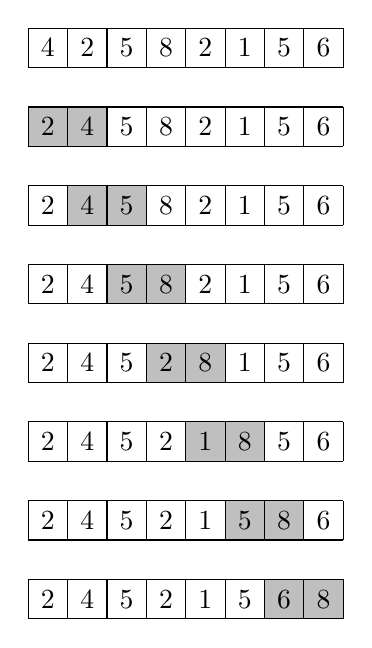
\begin{tikzpicture}[scale=0.5]
\begin{scope}
\draw (0,0) grid (8,1);
\foreach \x/\v in {0/4,1/2,2/5,3/8,4/2,5/1,6/5,7/6} \node at (0.5+\x,0.5) {\v};
\end{scope}
\begin{scope}[yshift=-2cm]
\fill[lightgray] (0,0) rectangle (2,1);
\draw (0,0) grid (8,1);
\foreach \x/\v in {0/2,1/4,2/5,3/8,4/2,5/1,6/5,7/6} \node at (0.5+\x,0.5) {\v};
\end{scope}
\begin{scope}[yshift=-4cm]
\fill[lightgray] (1,0) rectangle (3,1);
\draw (0,0) grid (8,1);
\foreach \x/\v in {0/2,1/4,2/5,3/8,4/2,5/1,6/5,7/6} \node at (0.5+\x,0.5) {\v};
\end{scope}
\begin{scope}[yshift=-6cm]
\fill[lightgray] (2,0) rectangle (4,1);
\draw (0,0) grid (8,1);
\foreach \x/\v in {0/2,1/4,2/5,3/8,4/2,5/1,6/5,7/6} \node at (0.5+\x,0.5) {\v};
\end{scope}
\begin{scope}[yshift=-8cm]
\fill[lightgray] (3,0) rectangle (5,1);
\draw (0,0) grid (8,1);
\foreach \x/\v in {0/2,1/4,2/5,3/2,4/8,5/1,6/5,7/6} \node at (0.5+\x,0.5) {\v};
\end{scope}
\begin{scope}[yshift=-10cm]
\fill[lightgray] (4,0) rectangle (6,1);
\draw (0,0) grid (8,1);
\foreach \x/\v in {0/2,1/4,2/5,3/2,4/1,5/8,6/5,7/6} \node at (0.5+\x,0.5) {\v};
\end{scope}
\begin{scope}[yshift=-12cm]
\fill[lightgray] (5,0) rectangle (7,1);
\draw (0,0) grid (8,1);
\foreach \x/\v in {0/2,1/4,2/5,3/2,4/1,5/5,6/8,7/6} \node at (0.5+\x,0.5) {\v};
\end{scope}
\begin{scope}[yshift=-14cm]
\fill[lightgray] (6,0) rectangle (8,1);
\draw (0,0) grid (8,1);
\foreach \x/\v in {0/2,1/4,2/5,3/2,4/1,5/5,6/6,7/8} \node at (0.5+\x,0.5) {\v};
\end{scope}
\end{tikzpicture}
\caption{Kuplajärjestämisen ensimmäinen kierros.}
\label{fig:kupjar}
\end{figure}


Kuva X näyttää esimerkin kuplajärjestämisen ensimmäisestä
kierroksesta.
Kuplajärjestämisen ominaisuutena on, että $k$ kierroksen
jälkeen taulukon $k$ suurinta alkiota ovat oikeilla paikoillaan
taulukon lopussa.
Niinpä $n$ kierroksen jälkeen koko taulukko on järjestyksessä.

Kuplajärjestämisen voi toteuttaa seuraavalla koodilla:

\begin{code}
for (int i = 0; i < n; i++) {
    for (int j = 0; j < n-1; j++) {
        if (taulu[i] > taulu[j]) {
            swap(taulu[i],taulu[j]);
        }
    }
}
\end{code}

Tässä merkintä \texttt{swap(a,b)} tarkoittaa,
että vaihdamme keskenään arvot \texttt{a} ja \texttt{b}.
Merkintä vastaa siis seuraavaa koodia:

\begin{code}
t = a;
a = b;
b = t;
\end{code}

Kuplajärjestäminen muodostuu $n$ kierroksesta,
joista jokainen käy läpi taulukon,
joten algoritmi vie aikaa $O(n^2)$.

\subsection{Lisäysjärjestäminen}

Lisäysjärjestäminen käy läpi taulukon vasemmalta oikealle
ja siirtää jokaisessa kohdassa olevaa alkiota vasemmalle
niin kauan kuin alkio on pienempi kuin sen vasemmalla
puolella oleva alkio.
Algoritmia voi myös ajatella niin,
että se varmistaa jokaisessa vaiheessa,
että taulukon $k$ ensimmäistä alkiota ovat oikeassa järjestyksessä.

\begin{figure}
\center
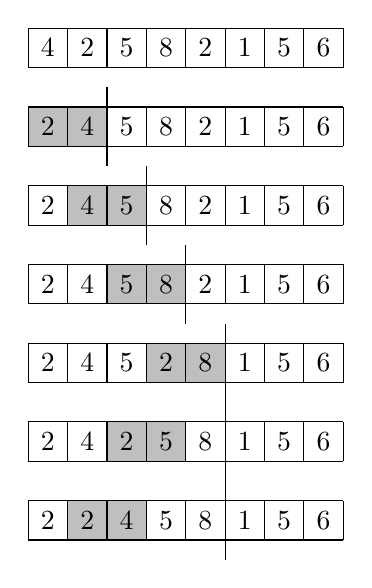
\begin{tikzpicture}[scale=0.5]
\begin{scope}
\draw (0,0) grid (8,1);
\foreach \x/\v in {0/4,1/2,2/5,3/8,4/2,5/1,6/5,7/6} \node at (0.5+\x,0.5) {\v};
\end{scope}
\begin{scope}[yshift=-2cm]
\fill[lightgray] (0,0) rectangle (2,1);
\draw (0,0) grid (8,1);
\foreach \x/\v in {0/2,1/4,2/5,3/8,4/2,5/1,6/5,7/6} \node at (0.5+\x,0.5) {\v};
\draw (2,-0.5) -- (2,1.5);
\end{scope}
\begin{scope}[yshift=-4cm]
\fill[lightgray] (1,0) rectangle (3,1);
\draw (0,0) grid (8,1);
\foreach \x/\v in {0/2,1/4,2/5,3/8,4/2,5/1,6/5,7/6} \node at (0.5+\x,0.5) {\v};
\draw (3,-0.5) -- (3,1.5);
\end{scope}
\begin{scope}[yshift=-6cm]
\fill[lightgray] (2,0) rectangle (4,1);
\draw (0,0) grid (8,1);
\foreach \x/\v in {0/2,1/4,2/5,3/8,4/2,5/1,6/5,7/6} \node at (0.5+\x,0.5) {\v};
\draw (4,-0.5) -- (4,1.5);
\end{scope}
\begin{scope}[yshift=-8cm]
\fill[lightgray] (3,0) rectangle (5,1);
\draw (0,0) grid (8,1);
\foreach \x/\v in {0/2,1/4,2/5,3/2,4/8,5/1,6/5,7/6} \node at (0.5+\x,0.5) {\v};
\draw (5,-0.5) -- (5,1.5);
\end{scope}
\begin{scope}[yshift=-10cm]
\fill[lightgray] (2,0) rectangle (4,1);
\draw (0,0) grid (8,1);
\foreach \x/\v in {0/2,1/4,2/2,3/5,4/8,5/1,6/5,7/6} \node at (0.5+\x,0.5) {\v};
\draw (5,-0.5) -- (5,1.5);
\end{scope}
\begin{scope}[yshift=-12cm]
\fill[lightgray] (1,0) rectangle (3,1);
\draw (0,0) grid (8,1);
\foreach \x/\v in {0/2,1/2,2/4,3/5,4/8,5/1,6/5,7/6} \node at (0.5+\x,0.5) {\v};
\draw (5,-0.5) -- (5,1.5);
\end{scope}
\end{tikzpicture}
\caption{Lisäysjärjestämisen ensimmäiset vaiheet.}
\label{fig:lisjar}
\end{figure}

Kuva \ref{fig:lisjar} näyttää esimerkin,
kuinka lisäysjärjestäminen aloittaa taulukon järjestämisen.
Jokaisessa kohdassa pystyviiva ilmaisee kohdan,
johon päättyy taulukon järjestyksessä oleva alkuosa.
Toisin kuin kuplajärjestämisessä, vierekkäisten alkioiden
vaihtamiset etenevät oikealta vasemmalle.

Seuraava koodi toteuttaa lisäysjärjestämisen:

\begin{code}
for (int i = 1; i < n; i++) {
    int k = i-1;
    while (k >= 0 && taulu[k] > taulu[k+1]) {
        swap(taulu[k],taulu[k+1]);
        k--;
    }
}
\end{code}

\subsection{Inversiot}

Kuplajärjestäminen ja lisäysjärjestäminen ovat esimerkkejä
järjestämis\-algoritmeista, jotka perustuvat vierekkäisten
alkioiden vaihtamiseen.
Osoitamme seuraavaksi, että tällainen algoritmi ei voi koskaan
toimia tehokkaammin kuin ajassa $O(n^2)$.

Hyödyllinen käsite järjestämisalgoritmien analysoinnissa
on \emph{inversio}: kaksi taulukossa olevaa alkiota,
jotka ovat väärässä järjestyksessä.
Tässä otetaan huomioon kaikki taulukon alkioparit,
ei vain vierekkäin olevia alkioita.
Esimerkiksi taulukossa $[3,1,4,2]$ on kolme inversiota:
$(3,1)$, $(3,2)$ ja $(4,2)$.

Taulukon inversioiden määrä kertoo, miten paljon työtä
vaaditaan sen järjestämiseen. Jos inversioiden määrä on 0,
taulukko on järjestyksessä.
Jos taas taulukko on käänteisessä järjestyksessä
suurimmasta pienimpään, sen inversioiden määrä on
\[
(n-1) + (n-2) + \dots + 1 = \frac{n(n-1)}{2} = O(n^2).
\]

Aina kun vaihdamme taulukossa kahden vierekkäin olevan
alkion järjes\-tyksen, saamme poistettua taulukosta enintään
yhden inversion.
Niinpä jos taulukossa on $O(n^2)$ inversiota,
mikä tahansa vierekkäisiä alkioita vaihtava algoritmi
käyttää sen järjestämiseen aikaa ainakin $O(n^2)$.
Emme siis koskaan pysty luomaan tehokasta järjestämisalgoritmia,
jos keskitymme vain algoritmeihin, jotka vaihtavat
keskenään vierekkäisiä alkioita.

\subsection{Vaihtojärjestäminen}

Vaihtojärjestäminen etsii ensin taulukon pienimmän alkion
ja vaihtaa sen ensimmäiseksi.
Tämän jälkeen se käsittelee vastaavasti taulukon
jäljellä olevan osan, jne., kunnes taulukko on järjestyksessä.
Kuva \ref{fig:vaijar} näyttää esimerkin
vaihtojärjestämisen toiminnasta.

\begin{figure}
\center
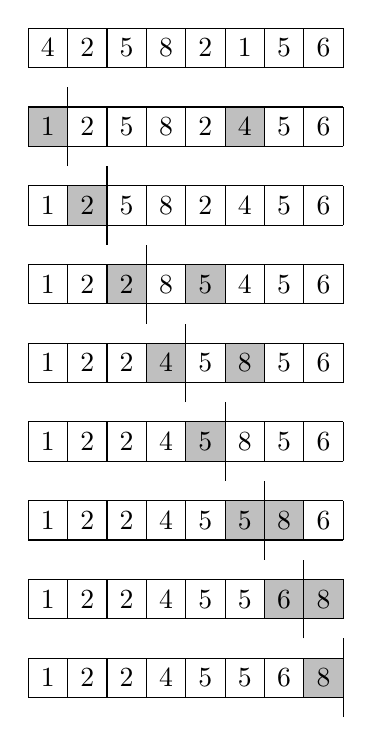
\begin{tikzpicture}[scale=0.5]
\begin{scope}
\draw (0,0) grid (8,1);
\foreach \x/\v in {0/4,1/2,2/5,3/8,4/2,5/1,6/5,7/6} \node at (0.5+\x,0.5) {\v};
\end{scope}
\begin{scope}[yshift=-2cm]
\fill[lightgray] (0,0) rectangle (1,1);
\fill[lightgray] (5,0) rectangle (6,1);
\draw (0,0) grid (8,1);
\foreach \x/\v in {0/1,1/2,2/5,3/8,4/2,5/4,6/5,7/6} \node at (0.5+\x,0.5) {\v};
\draw (1,-0.5) -- (1,1.5);
\end{scope}
\begin{scope}[yshift=-4cm]
\fill[lightgray] (1,0) rectangle (2,1);
\fill[lightgray] (1,0) rectangle (2,1);
\draw (0,0) grid (8,1);
\foreach \x/\v in {0/1,1/2,2/5,3/8,4/2,5/4,6/5,7/6} \node at (0.5+\x,0.5) {\v};
\draw (2,-0.5) -- (2,1.5);
\end{scope}
\begin{scope}[yshift=-6cm]
\fill[lightgray] (2,0) rectangle (3,1);
\fill[lightgray] (4,0) rectangle (5,1);
\draw (0,0) grid (8,1);
\foreach \x/\v in {0/1,1/2,2/2,3/8,4/5,5/4,6/5,7/6} \node at (0.5+\x,0.5) {\v};
\draw (3,-0.5) -- (3,1.5);
\end{scope}
\begin{scope}[yshift=-8cm]
\fill[lightgray] (3,0) rectangle (4,1);
\fill[lightgray] (5,0) rectangle (6,1);
\draw (0,0) grid (8,1);
\foreach \x/\v in {0/1,1/2,2/2,3/4,4/5,5/8,6/5,7/6} \node at (0.5+\x,0.5) {\v};
\draw (4,-0.5) -- (4,1.5);
\end{scope}
\begin{scope}[yshift=-10cm]
\fill[lightgray] (4,0) rectangle (5,1);
\fill[lightgray] (4,0) rectangle (5,1);
\draw (0,0) grid (8,1);
\foreach \x/\v in {0/1,1/2,2/2,3/4,4/5,5/8,6/5,7/6} \node at (0.5+\x,0.5) {\v};
\draw (5,-0.5) -- (5,1.5);
\end{scope}
\begin{scope}[yshift=-12cm]
\fill[lightgray] (5,0) rectangle (6,1);
\fill[lightgray] (6,0) rectangle (7,1);
\draw (0,0) grid (8,1);
\foreach \x/\v in {0/1,1/2,2/2,3/4,4/5,5/5,6/8,7/6} \node at (0.5+\x,0.5) {\v};
\draw (6,-0.5) -- (6,1.5);
\end{scope}
\begin{scope}[yshift=-14cm]
\fill[lightgray] (6,0) rectangle (7,1);
\fill[lightgray] (7,0) rectangle (8,1);
\draw (0,0) grid (8,1);
\foreach \x/\v in {0/1,1/2,2/2,3/4,4/5,5/5,6/6,7/8} \node at (0.5+\x,0.5) {\v};
\draw (7,-0.5) -- (7,1.5);
\end{scope}
\begin{scope}[yshift=-16cm]
\fill[lightgray] (7,0) rectangle (8,1);
\fill[lightgray] (7,0) rectangle (8,1);
\draw (0,0) grid (8,1);
\foreach \x/\v in {0/1,1/2,2/2,3/4,4/5,5/5,6/6,7/8} \node at (0.5+\x,0.5) {\v};
\draw (8,-0.5) -- (8,1.5);
\end{scope}
\end{tikzpicture}
\caption{Esimerkki vaihtojärjestämisen toiminnasta.}
\label{fig:vaijar}
\end{figure}


Seuraava koodi toteuttaa vaihtojärjestämisen:

\begin{code}
for (int i = 0; i < n; i++) {
    int k = i;
    for (int j = i; j < n; j++) {
        if (taulu[j] < taulu[k]) k = j;
    }
    swap(taulu[i],taulu[k]);
}
\end{code}

Toisin kuin kuplajärjestäminen ja lisäysjärjestäminen,
vaihtojärjestäminen vaihtaa vain $O(n)$ alkiota keskenään
taulukossa, koska se siirtää aina pienimmän alkion
suoraan oikeaan kohtaan.
Algoritmi vie kuitenkin $O(n^2)$ aikaa,
koska jokaisen pienimmän alkion löytäminen vie $O(n)$ aikaa.

Myöhemmin luvussa X huomaamme kuitenkin,
että voimme luoda vaihtojärjestämisen idealla tehokkaan
$O(n \log n)$-algoritmin käyttämällä apuna kekorakennetta.

\section{Tehokkaat algoritmit}

\subsection{Lomitusjärjestäminen}

\subsection{Pikajärjestäminen}

\subsection{Järjestämisen alaraja}

\subsection{Laskemisjärjestäminen}

\section{Järjestäminen Javassa}

Käytännössä ei ole yleensä hyvä idea toteuttaa itse
järjestämisalgoritmia, koska nykypäivän ohjelmointikielissä
on valmiit työkalut järjestämiseen.
Esimerkiksi Javassa voimme käyttää metodia \texttt{Arrays.sort},
joka järjestää sille annetun taulukon:

\begin{code}
int[] taulu = {4,2,5,8,2,1,5,6};
Arrays.sort(taulu);
\end{code}

Kiinnostava kysymys on, mitä algoritmia Java käyttää
taulukon järjes\-tämiseen.
Yllättävää kyllä, tämä riippuu siitä, minkä tyyppistä tietoa
taulukossa on.
Jos taulukon alkiot ovat alkeistyyppisiä
(esimerkiksi \texttt{int}), Java käyttää 
pikajärjestämisen muunnelmaa.
Jos taas alkiot ovat oliotyyppisiä
(esimerkiksi \texttt{String}),
algoritmina on lomitusjärjestäminen.

Jos haluamme, että Java pystyy järjestämään omia olioitamme,
meidän täytyy toteuttaa luokkaan metodi \texttt{compareTo} ja
merkitä, että luokka toteuttaa rajapinnan \texttt{Comparable}.
Kun \texttt{Arrays.sort} järjestää taulukon,
se kutsuu metodia \texttt{compareTo} aina, kun se haluaa selvittää
kahden alkion suuruusjärjestyksen.
Metodin tulee palauttaa negatiivinen arvo, nolla tai positiivinen arvo
sen mukaan, onko olio itse pienempi, yhtä suuri vai suurempi
kuin parametrina annettu olio.

Esimerkiksi seuraava koodi toteuttaa luokan \texttt{Piste},
johon voidaan tallentaa pisteen x- ja y-koordinaatit.
Luokassa on metodi \texttt{compareTo}, joka määrittelee,
että pisteet järjestetään ensisijaisesti x-koordinaatin ja
toissijaisesti y-koordinaatin mukaan.

\begin{code}
public class Piste implements Comparable<Piste> {
    public int x, y;

    public int compareTo(Piste p) {
        if (this.x != p.x) return this.x-p.x;
        else return this.y-p.y;
    }
}
\end{code}

Metodin \texttt{compareTo} avulla voimme myös konkreettisesti
tarkastella, mitä Java tekee järjestäessään taulukon.
Seuraava luokka sisältää vain yhden luvun,
mutta ilmoittaa meille aina, kun Java kutsuu
\texttt{compareTo}-funktiota:

\begin{code}
public class Luku implements Comparable<Luku> {
    public int luku;

    public int compareTo(Luku x) {
        System.out.println("vertailu: " + luku + " " + x.luku);
        return this.luku-x.luku;
    }
}
\end{code}

Esimerkiksi kun järjestettävänä taulukkona on $[4,1,3,2]$,
saamme tietää, että Java tekee seuraavat vertailut:

\begin{code}
vertailu: 1 4
vertailu: 3 1
vertailu: 3 4
vertailu: 3 1
vertailu: 2 3
vertailu: 2 1
\end{code}

\section{Esimerkkejä}
